\documentclass[border=10pt]{standalone}
\usepackage{tikz}
\usetikzlibrary{positioning}
\usetikzlibrary{shadings}
\usetikzlibrary{decorations.markings}
\usetikzlibrary{decorations.pathmorphing}
\usetikzlibrary{decorations.pathreplacing}
\usetikzlibrary{arrows.meta}
\usetikzlibrary{decorations.fractals}
\usetikzlibrary{matrix,positioning,quotes}
\usetikzlibrary{calc}
\usetikzlibrary{intersections}
\usepackage{tikzducks}

\begin{document}
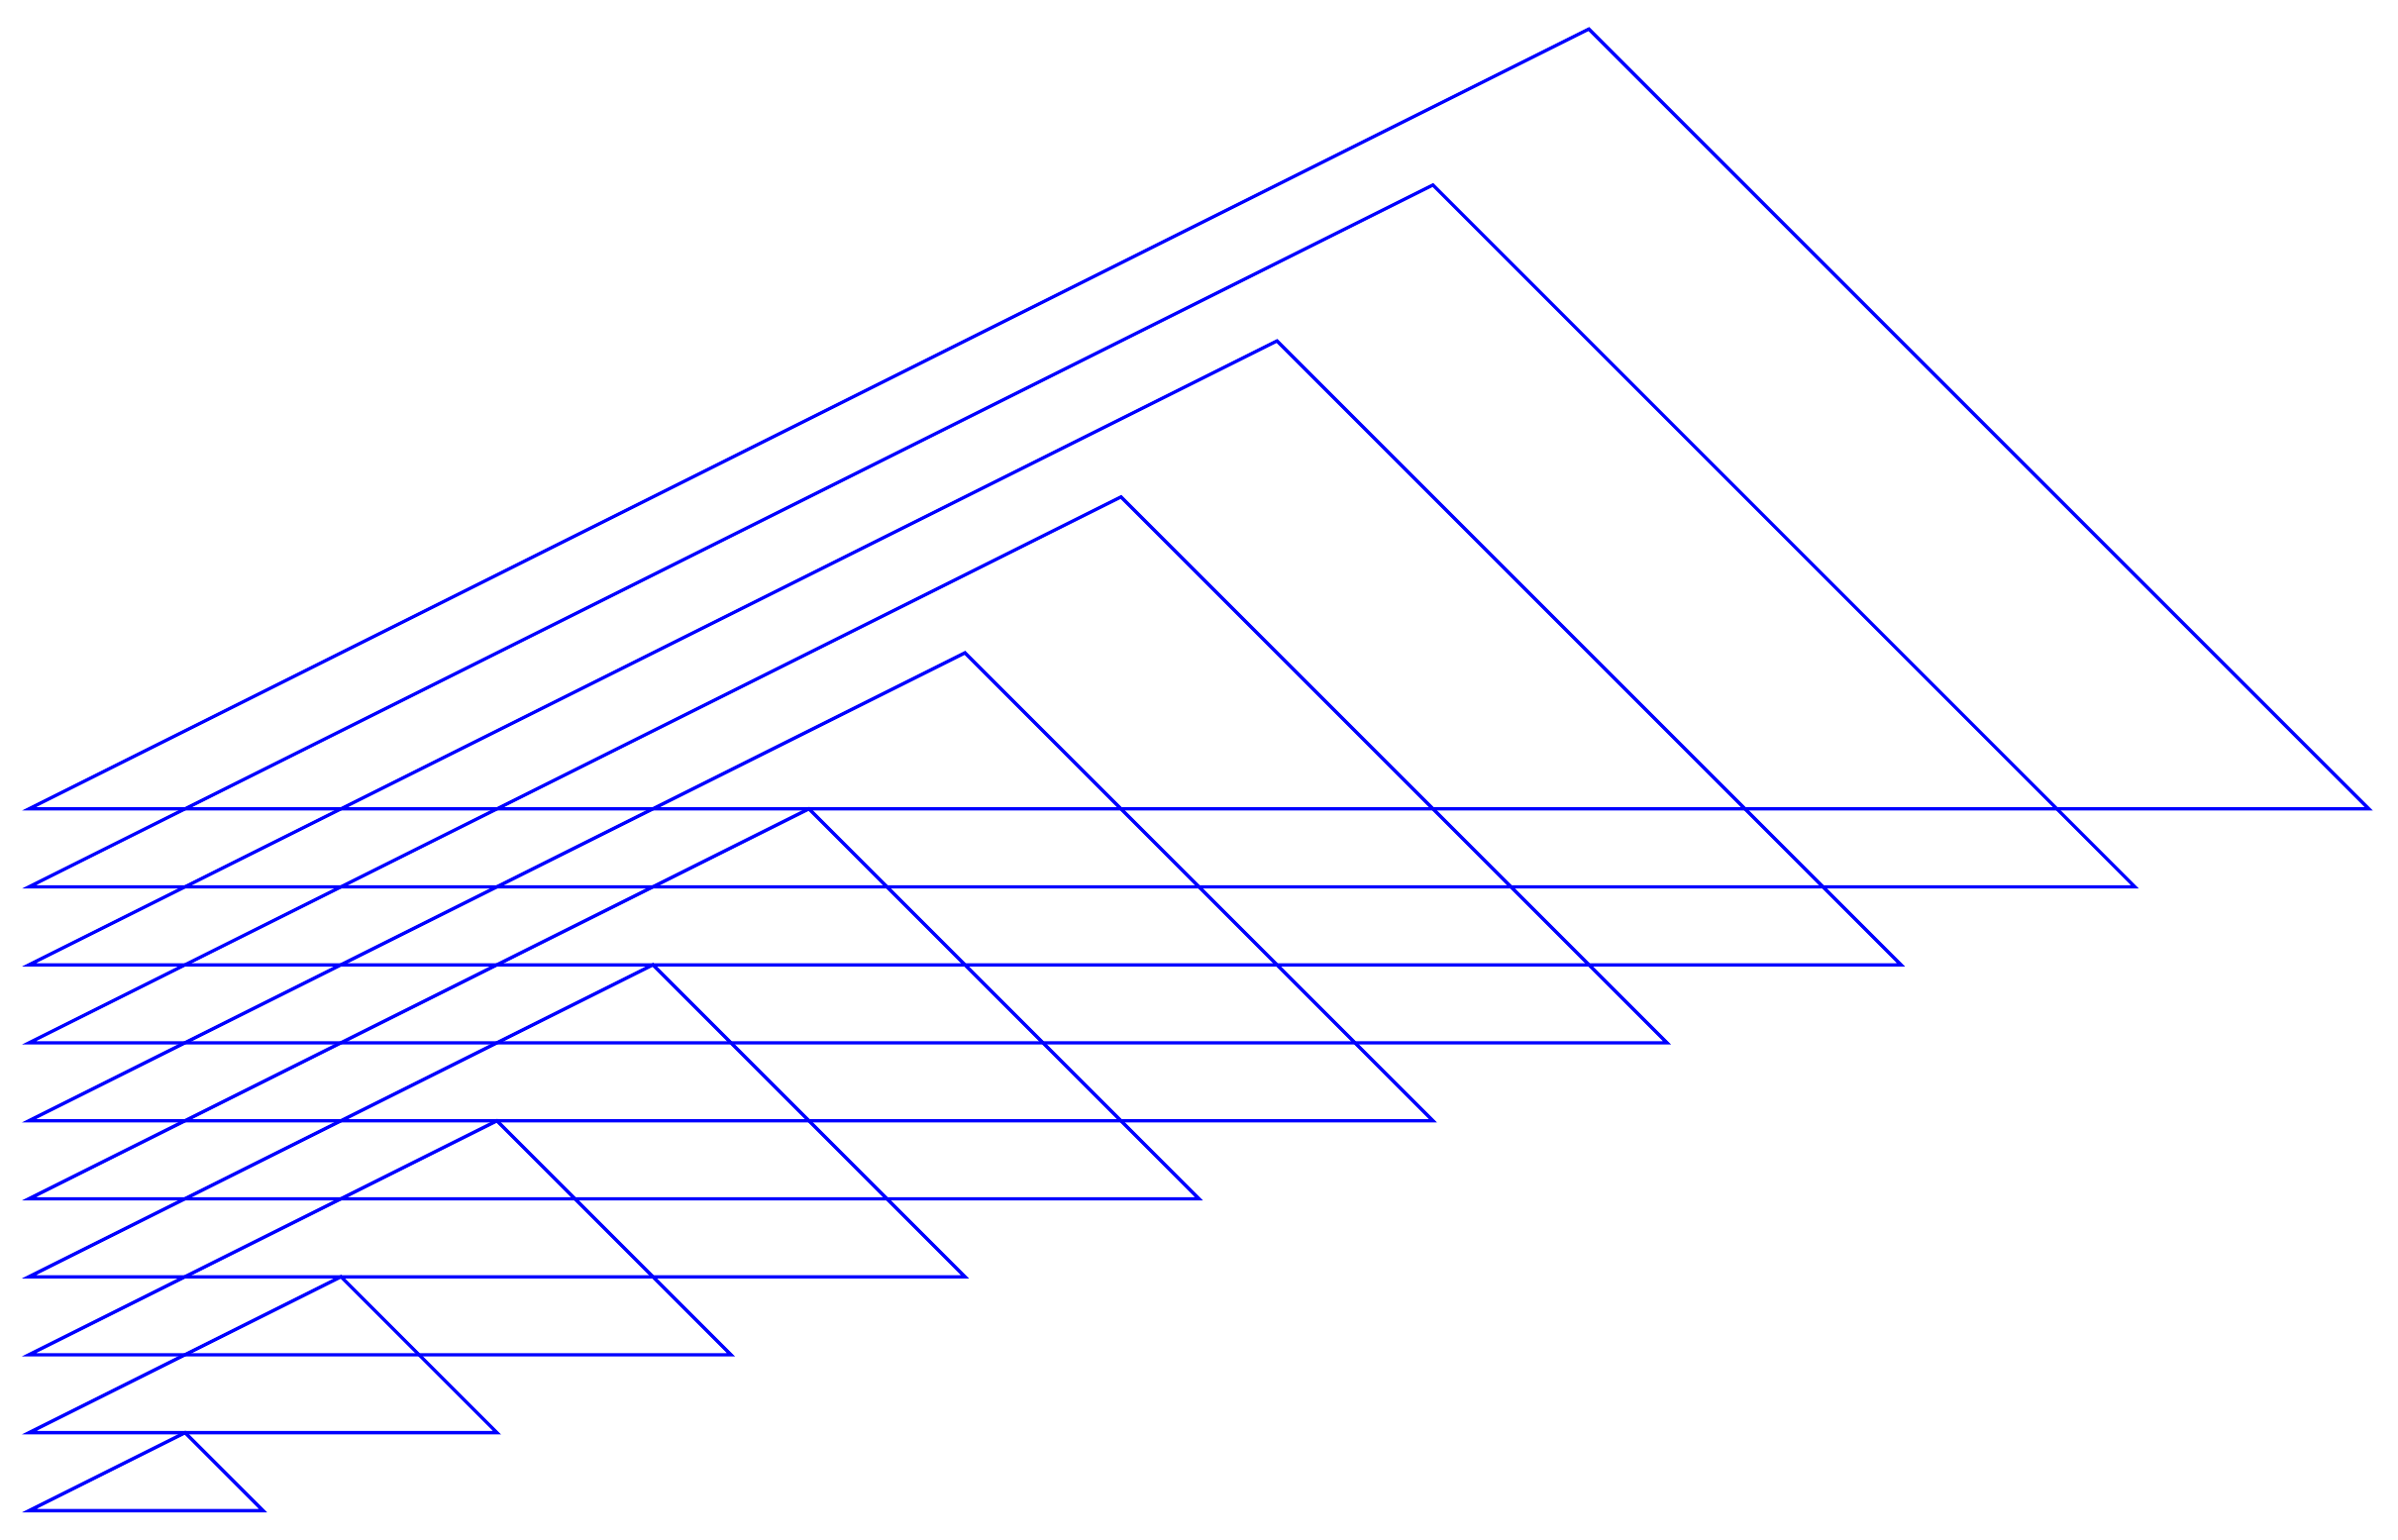
\begin{tikzpicture}
   \foreach \i in {1,2,3,...,10} \draw[scale=\i,very thick, color=blue] (0,1) -- (3,1) -- (2,2) --cycle; 
\end{tikzpicture}
\end{document}

